% =====================================================================
% VoiceShield: 8-page version of the paper (condensed from
% voiceshield_paper.tex, which is left unchanged). Same results, fewer
% words: no appendix, merged tables, the three most important figures.
% Single file, no .bib needed. Compile with pdfLaTeX (Overleaf default).
%
% Upload next to this file (same names as the long paper):
%   console.png    command center during a HOLD
%   customer.png   customer phone during the Step 9 attack (payment blocked)
%
% PAGE FIT: designed for 8 pages (A4, two columns) including references.
% If Overleaf shows a 9th page, set \screenshotsfalse below (saves about
% one third of a page); if it shows only 7, nothing needs to change.
% CHECK the author list and the references marked "verify".
% =====================================================================
\documentclass[10pt,a4paper,twocolumn]{article}

\usepackage[margin=18mm,columnsep=7mm,top=20mm,bottom=18mm]{geometry}
\usepackage[T1]{fontenc}
\usepackage[utf8]{inputenc}
\usepackage{mathptmx}
\usepackage{microtype}
\usepackage{graphicx}
\usepackage{adjustbox}
\usepackage{xcolor}
\usepackage{booktabs}
\usepackage{array}
\usepackage{amsmath}
\usepackage{amssymb}
\usepackage{caption}
\usepackage{titlesec}
\usepackage{fancyhdr}
\usepackage[authoryear,round]{natbib}
\usepackage{tikz}
\usetikzlibrary{arrows.meta,positioning}
\usepackage{pgfplots}
\pgfplotsset{compat=1.18}
\usepackage[colorlinks=true,linkcolor=black,citecolor=black,urlcolor=black]{hyperref}

\newif\ifscreenshots
\screenshotstrue   % \screenshotsfalse drops Figure 2 if the paper runs over 8 pages

\definecolor{seriesA}{HTML}{2A78D6}
\definecolor{seriesB}{HTML}{EB6834}
\definecolor{seriesC}{HTML}{1BAF7A}
\definecolor{gridgrey}{HTML}{E1E0D9}
\definecolor{inkmuted}{HTML}{52514E}

% screenshot helper: crop + scale, or a placeholder when the file is missing
\newcommand{\shotimg}[3]{%
  \IfFileExists{#2}%
  {\adjustbox{trim={#3},clip,width=#1}{\includegraphics{#2}}}%
  {\fbox{\parbox[c][2.4cm][c]{\dimexpr#1-2\fboxsep-2\fboxrule\relax}{\centering Image file not supplied}}}}

\DeclareCaptionLabelSeparator{bar}{ $\vert$ }
\captionsetup{labelsep=bar,labelfont=bf,font=footnotesize,justification=justified,singlelinecheck=false,skip=4pt}
\renewcommand{\figurename}{FIGURE}
\renewcommand{\tablename}{TABLE}
\setlength{\textfloatsep}{8pt plus 2pt minus 2pt}
\setlength{\floatsep}{6pt plus 2pt minus 2pt}
\setlength{\dbltextfloatsep}{8pt plus 2pt minus 2pt}
\setlength{\abovedisplayskip}{4pt}\setlength{\belowdisplayskip}{4pt}

\titleformat{\section}{\normalsize\bfseries\sffamily}{}{0em}{\MakeUppercase}
\titleformat{\subsection}{\small\bfseries\sffamily}{}{0em}{}
\titlespacing*{\section}{0pt}{7pt}{3pt}
\titlespacing*{\subsection}{0pt}{5pt}{2pt}
\setlength{\parindent}{1.1em}
\setlength{\parskip}{0pt}
\renewcommand{\arraystretch}{1.05}

\pagestyle{fancy}
\fancyhf{}
\fancyhead[R]{\small Real-Time Voice-Clone Impersonation Detection}
\fancyfoot[L]{\small VoiceShield}
\fancyfoot[R]{\small \thepage}
\renewcommand{\headrulewidth}{0.4pt}

\newcommand{\llr}{\ell}

\begin{document}

\twocolumn[
\begin{center}
{\sffamily\bfseries\Large VoiceShield: Real-Time Detection and Prevention of Voice-Cloning Impersonation in Calls, and Repairing a Self-Supervised Deepfake Detector Broken by Consumer Audio Processing Without Fine-Tuning\par}
\vspace{6pt}
% CHECK the author list for this project
{\normalsize Alapati Abhinav Chowdhary, Abhishek s, pendyala surya venkata sanjay\par}
\vspace{3pt}
{\small School of Computer Science and Engineering, Lovely Professional University, Phagwara, Punjab, India\par}
{\small Correspondence: \href{mailto:abhinavalapati.aac@gmail.com}{abhinavalapati.aac@gmail.com}\par}
\end{center}
\vspace{2pt}
\noindent\rule{\textwidth}{0.4pt}
\vspace{2pt}

\begin{minipage}{\textwidth}
\small
\noindent\textbf{Abstract.} Voice cloning lets a fraudster speak in the voice of a bank officer, a relative or the account holder.
We present VoiceShield, a prototype for the Smart India Hackathon 2026 problem SIH26104. It listens to a live call, returns PASS, VERIFY or HOLD every second, and blocks a pending bank transfer when the call is judged an impersonation.
It fuses three explainable signals:
a post-trained wav2vec~2.0 deepfake detector on 4-second windows;
a voiceprint check against an enrolled customer;
and multilingual scam-language rules on a Whisper transcript.
\emph{Zero-shot detector.} It separated same-speaker Hindi and Telugu clones (EER 0.0--0.1\%) and reached 4.7\% on an In-the-Wild sample, against 8.2\% on unseen premium commercial voices.
\emph{Consumer audio processing.} Processing applied before the detector is a major hidden failure mode.
Noise suppression raised the EER on premium clones to 34.0\%, and the Opus codec raised it to 45.1\%; Opus also flagged 32.7\% of genuine voices.
Operating-system microphone enhancements turned a genuine voice into a false alarm.
\emph{Fine-tuning.} Full fine-tuning and two LoRA methods, one anchored to the original model, all lost accuracy on real-world fakes.
\emph{Frozen-detector repair.} Keeping the detector frozen worked. Probes on its 25 layers showed that the middle blocks keep the evidence that the final read-out loses. A 1,050-parameter layer-weighted back-end, fused with the original head, reduced the mean EER over 13 unseen test sets from 9.7\% to 4.1\%, with no loss on In-the-Wild.
\emph{Live system.} The fused score turned two premium clones from VERIFY into HOLD while genuine callers passed.
\emph{Attack test.} A clone of the enrolled user's own voice nearly passed the voiceprint check (0.41 against a 0.45 cut-off). The detector still flagged every window, and the transfer requested in a live call was blocked.

\smallskip
\noindent\textbf{Keywords:} audio deepfake detection, voice cloning, anti-spoofing, self-supervised learning, wav2vec 2.0, layer-wise probing, speaker verification, scam detection, LoRA, robustness, real-time systems
\end{minipage}
\vspace{2pt}

\noindent\rule{\textwidth}{0.4pt}
\vspace{6pt}
]

% =====================================================================
\section{Introduction}
Text-to-speech (TTS) and voice-conversion (VC) systems can now imitate a person from a few seconds of public audio. In India this is used in ``digital arrest'' calls, fake bank calls that ask for a one-time password (OTP), and calls in the voice of a relative who needs money urgently. The Smart India Hackathon problem SIH26104 asks for a system that detects voice-cloning impersonation in real time and \emph{prevents} the attack, with a configurable risk engine, alerts, privacy-preserving logging and multilingual support (Smart India Hackathon, 2026).

Detecting synthetic speech is harder than benchmark accuracies suggest:
\begin{itemize}\setlength\itemsep{0pt}
\item detectors trained on one benchmark often fail on real-world fakes, with EERs of 34\% or more (M\"uller et al., 2022);
\item they can learn shortcuts such as the length of leading silence (M\"uller et al., 2021);
\item self-supervised (SSL) models such as wav2vec~2.0 (Baevski et al., 2020) generalise much better (Tak et al., 2022a), and post-training on tens of thousands of hours gives detectors that work zero-shot (Ge et al., 2025);
\item a call adds codecs, noise suppression and gain control before any detector hears the audio;
\item speaker verification alone fails because a good clone matches the target (Jung et al., 2022a).
\end{itemize}

Our contributions are:
\begin{itemize}\setlength\itemsep{0pt}
\item \textbf{(1)} A streaming system that fuses a synthetic-voice detector, a voiceprint and scam-language rules into an explainable PASS/VERIFY/HOLD decision, with a WebRTC call demonstrator that blocks payments.
\item \textbf{(2)} A measurement of how consumer audio processing (operating-system enhancements, noise suppression, auto-gain, Bluetooth and VoIP codecs) affects a strong detector, including false alarms on genuine speech.
\item \textbf{(3)} Three fine-tuning runs, including a teacher-anchored LoRA, all rejected because they forgot real-world fakes.
\item \textbf{(4)} A repair that keeps the detector frozen. Layer probes locate where the evidence survives, and a layer-weighted back-end halves the mean test EER without forgetting.
\item \textbf{(5)} Live and attack tests, including a clone of the enrolled person.
\end{itemize}

% =====================================================================
\section{Related Work}
\textbf{Generalisation.} The ASVspoof challenges (Wang et al., 2020; Liu et al., 2023; Wang et al., 2024) set the benchmarks for spoofed speech. Models trained on ASVspoof 2019 reach EERs of 34\% or more on In-the-Wild, real celebrity deepfakes (M\"uller et al., 2022). Deepfake-Eval-2024 found a large drop for open-source detectors on deepfakes circulated in 2024 (Chandra et al., 2025).

\textbf{SSL front ends.} Tak et al.\ (2022a) combined XLS-R (Babu et al., 2022) with AASIST (Jung et al., 2022b) and RawBoost (Tak et al., 2022b). Zhang et al.\ (2024) aggregated XLS-R layers with sensitive layer selection. A learned weighted sum of the layers of a frozen SSL model is the standard way to use such models downstream (Yang et al., 2021), and layer-wise probing shows that the blocks of wav2vec~2.0 encode different information (Pasad et al., 2021). Ge et al.\ (2025) post-trained SSL models on about 56k hours of real and 18k hours of fake speech (``AntiDeepfake''); the wav2vec~2.0 Large model reports 1.91\% EER on In-the-Wild. We use it as our detector.

\textbf{Channels.} RTCFake re-records speech through real-time communication platforms (RTCFake, 2026), and the RADAR 2026 challenge tests codecs, noise and reverberation (RADAR, 2026). We isolate effects that a phone, laptop or headset applies \emph{before} the call codec, and measure false alarms at a fixed threshold as well as EER.

\textbf{Verification and prevention.} SASV 2022 showed that a strong speaker verifier such as ECAPA-TDNN (Desplanques et al., 2020) is easily fooled by spoofed speech, and that fusing it with a countermeasure works best (Jung et al., 2022a). Watermarking (San Roman et al., 2024) and protective perturbation (Yu et al., 2023) do not stop an attacker with an open-source cloner, so we prevent at workflow level.

\textbf{Forgetting.} LoRA (Hu et al., 2022) learns a low-rank update of frozen weights. Fine-tuning on a small set can erase earlier knowledge (Kirkpatrick et al., 2017); Learning without Forgetting (Li and Hoiem, 2018) and distillation (Hinton et al., 2015) keep a model close to its earlier outputs.

% =====================================================================
\section{Methods}
\subsection{Detector Score and Metrics}
The detector maps a 4\,s waveform $x$ to logits $(z_{\text{fake}},z_{\text{real}})$. We use the log-odds score
\begin{equation}
\llr(x)=z_{\text{fake}}-z_{\text{real}},\qquad p_{\text{fake}}=\sigma(\llr),
\label{eq:llr}
\end{equation}
where positive means ``more likely fake'' and clean genuine speech scores near $-10$. With a threshold $\theta$, the false-alarm rate on genuine clips $\mathcal{R}$ and the miss rate on fakes $\mathcal{F}$ are
\begin{equation}
\mathrm{FAR}(\theta)=\tfrac{|\{i\in\mathcal{R}:\llr_i\geq\theta\}|}{|\mathcal{R}|},\quad
\mathrm{MR}(\theta)=\tfrac{|\{j\in\mathcal{F}:\llr_j<\theta\}|}{|\mathcal{F}|}.
\label{eq:far}
\end{equation}
The EER is the common value where they are equal, and measures ranking. Because a deployed system works at one threshold fixed in advance, we also report FAR and MR at a threshold calibrated on development data.

\subsection{Data}
Genuine speech is matched by fakes from the same speakers or channel where possible, so that a model cannot learn ``which data set is this'' (Table~\ref{tab:data}). All splits are by speaker. The Hume voices are used for development and the ElevenLabs and Kokoro voices for testing; none of these commercial voices is ever trained on.

\textbf{Same-speaker clones.} For 20 Kathbath speakers in each of Hindi and Telugu, we made 25 kNN-VC conversions per speaker from that speaker's own clips. This gives 500 genuine and 500 fake clips per language, split 14/3/3 speakers.

\textbf{Phone channel.} The phone version passes each clip through 300--3400\,Hz, 8\,kHz and G.711 $\mu$-law (ITU-T, 1988).

\textbf{Shortcut risk.} The clones sounded cleaner than the genuine clips. All training therefore applies the same noise and channel effects to both classes.

\begin{table}[t]
\centering\scriptsize
\caption{\textbf{Data.} kNN-VC clones were generated by us from each speaker's own clips.}
\label{tab:data}
\setlength{\tabcolsep}{3pt}
\begin{tabular}{@{}p{0.33\columnwidth}p{0.42\columnwidth}p{0.17\columnwidth}@{}}
\toprule
\textbf{Source} & \textbf{Content} & \textbf{Use}\\
\midrule
Kathbath (Javed et al., 2023) + kNN-VC (Baas et al., 2023) & Hindi, Telugu genuine speech and same-speaker clones & train, dev, test\\
IndicSynth (Sharma et al., 2025) & XTTS-v2, VITS, FreeVC clones & train, baseline\\
Commercial TTS (Stafford, 2025) & Polly, Speechify, Luvvoice (train); Hume (dev); ElevenLabs, Kokoro (test) & all\\
In-the-Wild (M\"uller et al., 2022) & real-world celebrity deepfakes & dev, test\\
Own recordings & laptop microphone (consent), ChatGPT voice, Windows-TTS scam script & live tests\\
\bottomrule
\end{tabular}
\end{table}

\subsection{Detector, Streaming and Line Profiles}
\textbf{Detector.} The detector is AntiDeepfake wav2vec~2.0 Large (Ge et al., 2025): a convolutional encoder, 24 transformer blocks (315\,M parameters), mean pooling and a linear head. It is served as ONNX on the laptop CPU with 4.0\,s windows, and the model's licence (CC BY-NC-SA) restricts use to non-commercial work.

\textbf{Streaming.} A FastAPI server receives 16-bit PCM over a WebSocket. Silero VAD v5 (Silero Team, 2024) keeps only speech, and after every 1\,s of new speech the last 4\,s are analysed. The detector, voiceprint and speech recogniser run in separate thread pools.

\textbf{Line profiles.} Scores depend on the channel, so every input line has its own threshold $\theta_\ell$:
\begin{itemize}\setlength\itemsep{0pt}
\item \texttt{default}: the pooled development EER;
\item \texttt{studio}: the EER on Hume development clips;
\item lines calibrated from genuine speech only, such as \texttt{mic}:
\begin{equation}
\theta_{\ell}=\mathrm{clip}\big(Q_{0.95}(\llr_{\text{genuine}})+1.5,\;-9.5,\;0\big).
\label{eq:calib}
\end{equation}
\end{itemize}

\subsection{Voiceprint, Scam Language and Risk Engine}
\textbf{Voiceprint.} WeSpeaker ResNet34 (Wang et al., 2023; Nagrani et al., 2017) gives window embeddings that are summed into a running voiceprint $\bar e$. The mismatch with the enrolled print $e_{\text{enr}}$ of the claimed person is $I=\sigma((0.45-\cos(\bar e,e_{\text{enr}}))/0.08)$. The cut-off of 0.45 lies between the within-speaker similarities we measured (0.60--0.87) and the between-speaker ones (0.00--0.25).

\textbf{Scam language.} Faster-whisper (Radford et al., 2023) transcribes each utterance. Rules for nine tactics, in English, Hindi and Telugu (romanised and native script), have weights $w_k$, and the tactics seen combine by noisy-OR:
\begin{equation}
C=1-\textstyle\prod_{k}(1-w_k).
\label{eq:scam}
\end{equation}
The tactics and weights are: OTP or PIN 0.6, remote-access app 0.5, money transfer 0.4, police threat 0.4, account block 0.35, family emergency 0.35, prize 0.3, urgency or secrecy 0.25, and bank or official claim 0.2.

\textbf{Risk engine.} Each window gives a score $s_t=\sigma(\llr_t-\theta_\ell)$, and the voice risk is a running average that starts at genuine, $V_t=0.6V_{t-1}+0.4s_t$ with $V_0=0$.
\begin{itemize}\setlength\itemsep{0pt}
\item \textbf{HOLD} if $V\geq75$ and 3 of the last 5 windows have $s\geq0.5$;
\item \textbf{HOLD} if $C\geq50$ and the voice or the identity was suspicious earlier in the call;
\item \textbf{VERIFY} if $V\geq45$, 2 of 5 windows are suspicious, $I\geq50$ or $C\geq50$;
\item \textbf{PASS} otherwise.
\end{itemize}
The verdict only escalates, a matching voice never lowers the risk, and every alert states its reasons in plain words.

\begin{figure*}[t]
\centering
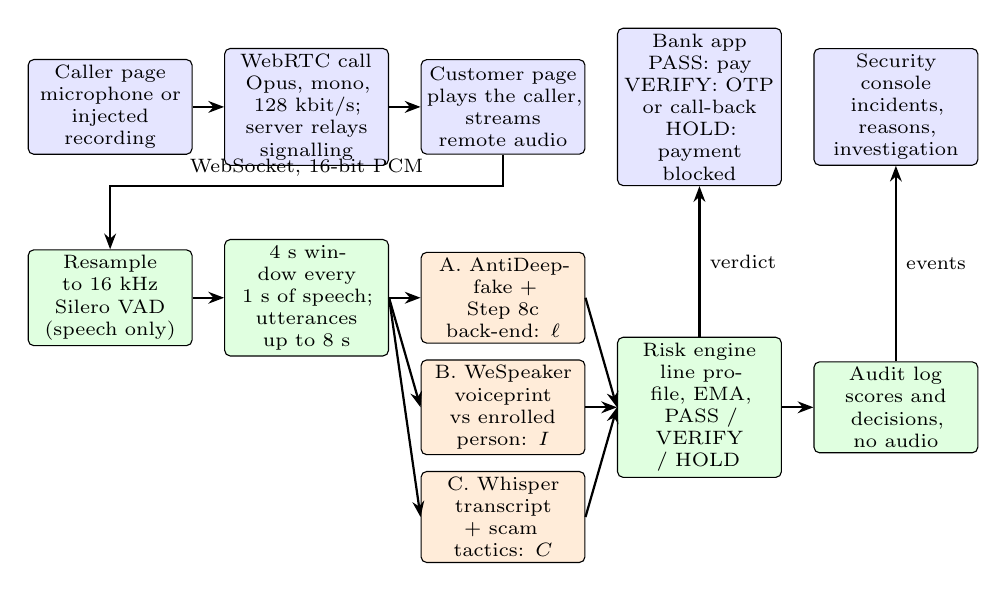
\begin{tikzpicture}[
  box/.style={draw,rounded corners=2pt,align=center,font=\scriptsize,text width=0.16\textwidth,minimum height=10mm,inner sep=2pt},
  web/.style={box,fill=blue!10,minimum height=12mm},
  srv/.style={box,fill=green!12},
  sig/.style={box,fill=orange!15,minimum height=8mm},
  arr/.style={-{Stealth[length=2mm]},thick}]
\node[web] (a1) {Caller page\\microphone or\\injected recording};
\node[web,right=4mm of a1] (a2) {WebRTC call\\Opus, mono, 128 kbit/s;\\server relays signalling};
\node[web,right=4mm of a2] (a3) {Customer page\\plays the caller,\\streams remote audio};
\node[web,right=4mm of a3] (a4) {Bank app\\PASS: pay\\VERIFY: OTP or call-back\\HOLD: payment blocked};
\node[web,right=4mm of a4] (a5) {Security console\\incidents, reasons,\\investigation};
\node[srv,below=12mm of a1] (b1) {Resample to 16 kHz\\Silero VAD\\(speech only)};
\node[srv,right=4mm of b1] (b2) {4 s window every\\1 s of speech;\\utterances up to 8 s};
\node[sig,right=4mm of b2] (b3) {A. AntiDeepfake +\\Step 8c back-end: $\llr$};
\node[sig,below=2mm of b3] (b4) {B. WeSpeaker voiceprint\\vs enrolled person: $I$};
\node[sig,below=2mm of b4] (b5) {C. Whisper transcript\\+ scam tactics: $C$};
\node[srv,right=4mm of b4] (b6) {Risk engine\\line profile, EMA,\\PASS / VERIFY / HOLD};
\node[srv,right=4mm of b6] (b7) {Audit log\\scores and decisions,\\no audio};
\draw[arr] (a1) -- (a2);
\draw[arr] (a2) -- (a3);
\draw[arr] (a3.south) -- ++(0,-4mm) -| node[pos=0.25,above,font=\scriptsize] {WebSocket, 16-bit PCM} (b1.north);
\draw[arr] (b1) -- (b2);
\draw[arr] (b2.east) -- (b3.west);
\draw[arr] (b2.east) -- (b4.west);
\draw[arr] (b2.east) -- (b5.west);
\draw[arr] (b3.east) -- (b6.west);
\draw[arr] (b4.east) -- (b6.west);
\draw[arr] (b5.east) -- (b6.west);
\draw[arr] (b6) -- (b7);
\draw[arr] (b6.north) -- node[right,font=\scriptsize] {verdict} (a4.south);
\draw[arr] (b7.north) -- node[right,font=\scriptsize] {events} (a5.south);
\end{tikzpicture}
\caption{\textbf{System overview.} Blue: call demonstrator pages. Green: server stages. Orange: the three independent signals. The customer's page streams the audio it \emph{receives}, so the system hears what the victim hears.}
\label{fig:overview}
\end{figure*}

\subsection{Call Demonstrator and Console}
\textbf{The call.} A \texttt{/caller} page, either the genuine caller or an attacker who \emph{injects a recording into the call}, and a \texttt{/customer} page are connected by WebRTC (W3C, 2021). The Opus codec (Valin et al., 2012) is set to mono at 128\,kbit/s without discontinuous transmission (Figure~\ref{fig:overview}).

\textbf{Prevention.}
\begin{itemize}\setlength\itemsep{0pt}
\item PASS allows payments.
\item VERIFY requires an OTP to the customer's registered phone, or a call-back on the official number.
\item HOLD blocks payments automatically and alerts the security team.
\end{itemize}

\textbf{The console.} A single-page console serves the operator and the security team. It has a live command center, a forensic voice analysis (waveform, spectrogram and per-window verdicts), incidents, history, an investigation view that keeps prediction, evidence and actions apart, analytics, and settings. Its live waveform is drawn from the same PCM chunks sent to the detector (Figure~\ref{fig:ui}).

\textbf{Privacy.} Only scores, decisions and the names of scam tactics are stored. Audio, transcripts and voiceprint recordings never are.

\ifscreenshots
\begin{figure*}[t]
\centering
\begin{minipage}[t]{0.495\textwidth}\centering
\shotimg{\linewidth}{console.png}{0pt 0pt 0pt 0pt}\\[1pt]
{\scriptsize (a) Command center during the demo scam call: HOLD at 4.4 s}
\end{minipage}\hfill
\begin{minipage}[t]{0.495\textwidth}\centering
\shotimg{\linewidth}{customer.png}{0pt 0pt 0pt 0pt}\\[1pt]
{\scriptsize (b) Customer phone during the Step 9 attack: the Rs.~49,999 payment is blocked}
\end{minipage}
\caption{\textbf{Screenshots captured from the running system.} Verdicts carry an icon and a word, never colour alone.}
\label{fig:ui}
\end{figure*}
\fi

\subsection{Consumer Processing Study and Fine-Tuning (Steps 4, 8, 8b)}
\textbf{Processing effects.} We implemented seven effects that devices and apps apply:
\begin{itemize}\setlength\itemsep{0pt}
\item noise suppression by spectral gating (Sainburg et al., 2020);
\item spectral subtraction (Boll, 1979);
\item automatic gain control, alone and followed by spectral subtraction;
\item a G.711 phone line;
\item Bluetooth CVSD at 8\,kHz;
\item an mSBC-like 16\,kHz channel;
\item Opus at 8--24\,kbit/s.
\end{itemize}
In the test sets each effect follows 15\,dB background noise.

\textbf{Step 4: full fine-tuning.} 3,760 clips, identical augmentation for both classes, backbone learning rate $5\times10^{-6}$.

\textbf{Step 8: LoRA, attempt 1.} LoRA ($r=8$, $\alpha=16$) on all attention and feed-forward projections: 3.54\,M of 319\,M parameters. Trained on 4,360 clips with processing augmentation.

\textbf{Step 8b: LoRA, attempt 2.} The same set-up, with the frozen original $f_0$ as a teacher on the clean crop $x$. The adapted model $f_\phi$ sees a processed copy $\tilde x$ and is trained with
\begin{equation}
\mathcal{L}=\mathrm{CE}(f_\phi(\tilde x),y)+\lambda\tau^{2}g\,\mathrm{KL}\big(\sigma_\tau(f_0(x))\,\Vert\,\sigma_\tau(f_\phi(\tilde x))\big),
\label{eq:consistency}
\end{equation}
with $\lambda=1$ and $\tau=2$. The gate $g=1$ only when the teacher is right.

\textbf{Model selection.} All runs were selected on development sets that include unseen Hume voices and In-the-Wild, with the original model as a candidate at step~0.

\subsection{Frozen-Detector Back-End (Step 8c)}
\textbf{Features.} Step 8c keeps every weight of the detector fixed. For each of its 25 hidden layers we take the time-mean $\bar h_l(x)$, standardised with training statistics:
\begin{equation}
z_l(x)=\big(\bar h_l(x)-\mu_l\big)/s_l,\qquad l=0,\dots,24,
\label{eq:layers}
\end{equation}
where layer 24 is what the original head reads.

\textbf{Training data.} Each of the 4,360 training clips gives one clean and two processed views (13,080 in all), with the processing type kept as a label.

\textbf{Layer probes.} A logistic-regression probe on each layer shows where the evidence survives processing.

\textbf{Back-end.} The back-end weights the layers and reads them out linearly (1,050 parameters), in the spirit of SUPERB (Yang et al., 2021) and SLS (Zhang et al., 2024):
\begin{equation}
q(x)=\mathbf{v}^{\top}\textstyle\sum_{l}\pi_l z_l(x)+b,\qquad \boldsymbol{\pi}=\mathrm{softmax}(\mathbf{a}).
\label{eq:backend}
\end{equation}

\textbf{Fusion.} It is fused with the original score as $f=(1-w)\,\hat\llr+w\,\hat q$, where both are standardised on development data. The weight $w\in\{0,0.05,\dots,1\}$ is chosen by mean development EER; at $w=0$ this is the original detector.

\textbf{Automatic line profile.} A second model of the same form, with 9 outputs, predicts the processing type, and the threshold calibrated for that type is used.

\textbf{Serving.} The live server uses an ONNX export with the layer outputs, a NumPy back-end, and the fused score on the $\llr$ scale with its own line profiles.

% =====================================================================
\section{Results}
\subsection{Zero-Shot Detector and Fine-Tuning}
\textbf{Baseline (Table~\ref{tab:zeroshot}).}
\begin{itemize}\setlength\itemsep{0pt}
\item AntiDeepfake reached 4.0\% EER on our In-the-Wild sample, close to the published 1.91\% given our 4\,s crops. This suggests our pipeline is correct.
\item A popular Hugging Face classifier scored 32--38\% outside its own training data.
\item On same-speaker clones, AntiDeepfake was nearly perfect. The phone line was the first weakness: the Telugu EER rose from 0.0\% to 5.2\%, and the best threshold fell from 0.34--0.88 to 0.05--0.08.
\item Premium commercial voices were the main weak spot: 8.2\% EER, and 15.0\% over a phone line.
\end{itemize}
\textbf{Step 4 fine-tuning.} It improved the unseen Hume voices but raised the In-the-Wild development EER to 7.0--8.5\%. Model selection kept the original.

\begin{table}[t]
\centering\scriptsize
\caption{\textbf{Zero-shot detectors on unseen sets} (EER \%). A: AntiDeepfake. B: a wav2vec~2.0 classifier fine-tuned on the commercial set (its 1.3\% there is invalid: own training data).}
\label{tab:zeroshot}
\setlength{\tabcolsep}{3pt}
\begin{tabular}{@{}p{0.56\columnwidth}rr@{}}
\toprule
\textbf{Test set} & \textbf{A} & \textbf{B}\\
\midrule
Hindi, Kathbath vs IndicSynth (Step 2) & 0.0 & 32.0\\
Commercial TTS (Step 2) & 10.0 & (1.3)\\
In-the-Wild sample (Step 2 / test sample) & 4.0 / 4.7 & 37.7\\
Hindi / Telugu same-speaker kNN-VC, clean & 0.1 / 0.0 & --\\
Hindi / Telugu same-speaker kNN-VC, phone & 1.5 / 5.2 & --\\
Premium ElevenLabs + Kokoro, clean / phone & 8.2 / 15.0 & --\\
\bottomrule
\end{tabular}
\end{table}

\subsection{Live Pipeline, Calls and Input Devices}
\textbf{Latency.} On the laptop CPU the detector takes 330\,ms per window, so a 1\,s hop runs in real time. Whisper small transcribes 8\,s of speech in 0.2--0.3\,s on the laptop GPU (Table~\ref{tab:live}).

\textbf{Demo calls and live tests.}
\begin{itemize}\setlength\itemsep{0pt}
\item With the original detector, genuine demo callers passed. Premium clones reached VERIFY or a late HOLD on voice alone.
\item A Windows-TTS scam script reached HOLD after 4.4\,s, with four tactics recognised.
\item When a team member and ChatGPT's voice read the same script, the AI voice was held after 5.3\,s (31 of 45 windows flagged) and the human passed (0 of 19).
\item In a two-browser WebRTC call, an injected scam recording was held after about 4\,s of speech and a Rs.~49,999 transfer was blocked automatically.
\end{itemize}

\textbf{Input devices.} The input device mattered more than the model. A Bluetooth or virtual default input scored genuine speech at $\llr=+2.2$. With Windows microphone enhancements on, the score was $-2.3$, a false HOLD that also varied between sessions. With the enhancements off it was $-10.0$. We therefore calibrate the raw microphone (Equation~\ref{eq:calib}; \texttt{mic} $=-6.01$).

\begin{table}[t]
\centering\scriptsize
\caption{\textbf{Live tests, original detector.} Times are seconds of speech after the voice starts.}
\label{tab:live}
\setlength{\tabcolsep}{3pt}
\begin{tabular}{@{}p{0.55\columnwidth}p{0.37\columnwidth}@{}}
\toprule
\textbf{Test} & \textbf{Result}\\
\midrule
Two genuine demo callers, team member's voice & PASS\\
ElevenLabs / Kokoro clone, voice only (\texttt{studio}) & VERIFY 3.2 s / HOLD 16.5 s\\
Windows-TTS scam script (OTP, account block) & HOLD 4.4 s, scam score 84\\
Same script: ChatGPT voice vs. human & HOLD 5.3 s vs. PASS\\
Injected scam call through WebRTC & HOLD $\approx$4 s, transfer blocked\\
Genuine voice, enhancements on / off & false HOLD ($-2.3$) / PASS ($-10.0$)\\
\bottomrule
\end{tabular}
\end{table}

\subsection{Consumer Processing Breaks the Detector}
Table~\ref{tab:dsp} gives the original detector on the unseen test sets.

\textbf{Premium clones are laundered.} Noise suppression raised their EER from 8.2\% to 34.0\% (AUC 0.70), and Opus raised it to 45.1\% (AUC 0.59).

\textbf{Opus shifts genuine speech.} It flagged 32.7\% of genuine Indian-language clips (49 of 150; Wilson interval 25.7--40.5\%; Wilson, 1927), although the EER stayed at 4.7\%.

\textbf{Bluetooth CVSD hides even kNN-VC clones.} The EER rose from 0.0\% to 10.0\%, with 26.7\% of fakes missed.

\textbf{Two LoRA attempts.} Both learned the processed conditions: CVSD development EER 14.0\% to 10.7\% and 11.3\%. Both lost real-world fakes: In-the-Wild development EER 4.0\% to 9.5\%. The anchor of attempt~2 was active (the teacher was right on 92--96\% of crops), yet it did not hold In-the-Wild in place (Table~\ref{tab:ft}).

\begin{table*}[t]
\centering\footnotesize
\caption{\textbf{Consumer processing (Step 8) and the frozen-detector back-end (Step 8c) on unseen test sets.} Processing is applied after 15\,dB noise. FAR / MR: genuine flagged / fakes missed at the development threshold, original detector. Fused: $f=(1-w)\hat\llr+w\hat q$ with $w=0.85$ chosen on development data. Premium = ElevenLabs + Kokoro.}
\label{tab:dsp}
\setlength{\tabcolsep}{5pt}
\begin{tabular}{@{}llrrrrrrr@{}}
\toprule
 & & \multicolumn{4}{c}{\textbf{Original detector}} & \multicolumn{3}{c}{\textbf{Step 8c}}\\
\cmidrule(lr){3-6}\cmidrule(l){7-9}
\textbf{Test set} & \textbf{Processing} & \textbf{EER \%} & \textbf{AUC} & \textbf{FAR \%} & \textbf{MR \%} & \textbf{Back-end EER} & \textbf{Fused EER} & \textbf{Fused AUC}\\
\midrule
Hindi, Telugu test speakers & clean & 0.0 & 1.000 & 0.7 & 0.0 & 0.0 & 0.0 & 1.000\\
 & phone line (G.711) & 2.0 & 0.995 & 4.7 & 2.7 & 0.0 & 0.0 & 1.000\\
 & noise suppression & 5.0 & 0.988 & 4.7 & 6.0 & 1.3 & 1.3 & 1.000\\
 & spectral subtraction & 1.3 & 0.992 & 1.3 & 1.3 & 0.3 & 0.3 & 1.000\\
 & auto-gain + spectral subtraction & 2.0 & 0.998 & 3.3 & 0.7 & 1.0 & 1.3 & 1.000\\
 & Bluetooth CVSD & \textbf{10.0} & 0.953 & 1.3 & \textbf{26.7} & 3.3 & 4.0 & 0.991\\
 & Bluetooth mSBC-like & 2.0 & 0.996 & 2.7 & 2.7 & 0.0 & 0.0 & 1.000\\
 & Opus & 4.7 & 0.989 & \textbf{32.7} & 0.0 & 0.0 & 1.3 & 1.000\\
\midrule
Premium commercial & clean & 8.2 & 0.956 & 0.4 & 51.0 & 3.4 & 3.0 & 0.989\\
 & noise suppression & \textbf{34.0} & 0.699 & 0.9 & \textbf{72.6} & 11.2 & 12.7 & 0.946\\
 & Opus & \textbf{45.1} & 0.589 & 32.6 & 58.1 & 14.1 & 16.7 & 0.890\\
\midrule
In-the-Wild sample & clean & 4.7 & 0.992 & 4.7 & 5.7 & 4.7 & 4.7 & 0.986\\
 & noise suppression & 7.5 & 0.974 & 5.0 & 12.3 & 7.7 & 7.3 & 0.976\\
\midrule
\multicolumn{2}{@{}l}{\textbf{Mean of the 13 test sets} (10 processed sets)} & \textbf{9.73} (11.36) & & & & \textbf{3.62} (3.90) & \textbf{4.05} (4.50) & \\
\bottomrule
\end{tabular}
\end{table*}

\begin{table}[t]
\centering\scriptsize
\caption{\textbf{Changing the detector vs. keeping it frozen.} Development EER at each method's best checkpoint (8 sets; Step 4: 4 sets).}
\label{tab:ft}
\setlength{\tabcolsep}{3pt}
\begin{tabular}{@{}p{0.38\columnwidth}rrrl@{}}
\toprule
\textbf{Method} & \textbf{Trained} & \textbf{Dev mean} & \textbf{ITW dev} & \textbf{Kept}\\
\midrule
Original detector & -- & 4.17 & 4.0 & baseline\\
Full fine-tuning (Step 4) & 315 M & 2.65* & 7.0--8.5 & no\\
LoRA (Step 8) & 3.54 M & 5.28 & 9.5 & no\\
LoRA + teacher (Step 8b) & 3.54 M & 5.79 & 8.3 & no\\
\textbf{Frozen + back-end (8c)} & \textbf{1,050} & \textbf{1.39} & --$^\dagger$ & \textbf{yes}\\
\bottomrule
\end{tabular}\\[1pt]
{\scriptsize *4-set mean; the original scored 1.50 on those sets. ITW: In-the-Wild. $^\dagger$Not logged separately; on the In-the-Wild test sample it stayed at the original's 4.67.}
\end{table}

\subsection{The Frozen-Detector Repair (Step 8c)}
\textbf{Where the evidence survives (Figure~\ref{fig:layers}).}
\begin{itemize}\setlength\itemsep{0pt}
\item From block 5 on, the layer probes reach 1.7--2.0\% mean development EER and 4.2--4.5\% mean test EER.
\item Blocks 21--23 lose the evidence under CVSD (9.0--11.3\%).
\item A probe on the last layer alone reaches 6.6\% mean test EER, against 9.7\% for the original head. Much of the damage is therefore in the read-out, not in the representation.
\item The back-end found the same pattern on its own: its largest weights are on blocks 9--11.
\end{itemize}

\textbf{Back-end and fusion.} The back-end reached 1.51\% mean development EER, and fusion ($w=0.85$) 1.39\%.

\textbf{Unseen test sets (Table~\ref{tab:dsp}).}
\begin{itemize}\setlength\itemsep{0pt}
\item The mean EER over 13 sets fell from 9.73\% to 4.05\%.
\item Premium clones improved even without processing: 8.2\% to 3.0\%.
\item Under noise suppression they fell from 34.0\% to 12.7\%, and under Opus from 45.1\% to 16.7\% (AUC 0.59 to 0.89).
\item In-the-Wild, where every fine-tuning run had lost accuracy, stayed at 4.67\%.
\end{itemize}

\begin{figure}[t]
\centering
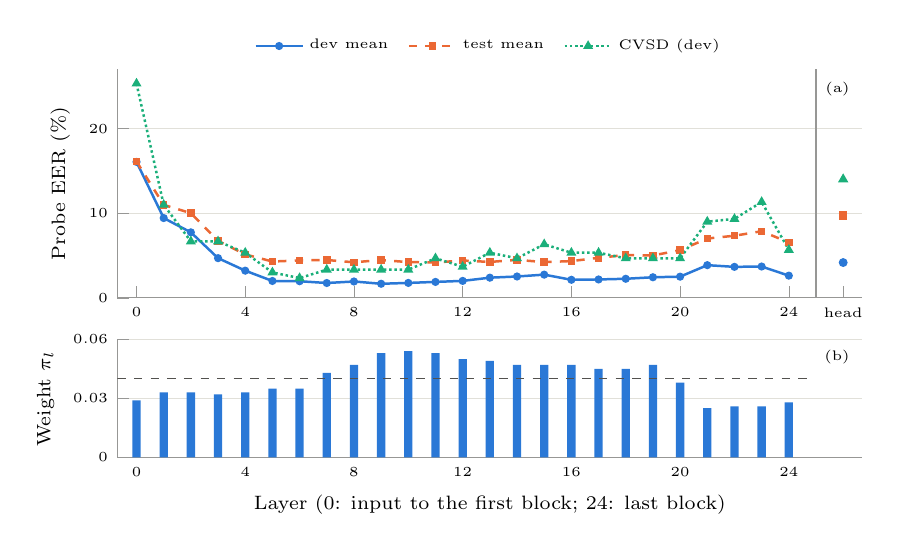
\begin{tikzpicture}
\begin{axis}[
  name=top, scale only axis, width=0.78\columnwidth, height=2.9cm,
  xmin=-0.7, xmax=26.7, ymin=0, ymax=27,
  xtick={0,4,8,12,16,20,24,26}, xticklabels={0,4,8,12,16,20,24,head}, ytick={0,10,20},
  ylabel={Probe EER (\%)},
  tick label style={font=\tiny}, label style={font=\scriptsize},
  axis lines*=left, axis line style={inkmuted!60}, tick style={inkmuted!60},
  ymajorgrids, grid style={gridgrey},
  legend style={font=\tiny, draw=none, fill=none, at={(0.5,1.02)}, anchor=south, legend columns=3,
    /tikz/every even column/.append style={column sep=5pt}},
  legend cell align=left,
]
\addplot[seriesA, line width=0.9pt, mark=*, mark size=1pt] coordinates {
(0,16.07) (1,9.43) (2,7.74) (3,4.69) (4,3.21) (5,1.99) (6,1.96) (7,1.75) (8,1.93) (9,1.66) (10,1.76) (11,1.88) (12,2.00)
(13,2.38) (14,2.52) (15,2.74) (16,2.13) (17,2.17) (18,2.25) (19,2.43) (20,2.50) (21,3.86) (22,3.66) (23,3.70) (24,2.62)};
\addlegendentry{dev mean}
\addplot[seriesB, line width=0.9pt, dashed, mark=square*, mark size=0.9pt, mark options={solid}] coordinates {
(0,16.12) (1,10.99) (2,10.01) (3,6.73) (4,5.13) (5,4.29) (6,4.42) (7,4.47) (8,4.20) (9,4.47) (10,4.22) (11,4.18) (12,4.41)
(13,4.24) (14,4.49) (15,4.22) (16,4.34) (17,4.73) (18,5.06) (19,5.01) (20,5.63) (21,7.01) (22,7.34) (23,7.87) (24,6.55)};
\addlegendentry{test mean}
\addplot[seriesC, line width=0.9pt, densely dotted, mark=triangle*, mark size=1.2pt, mark options={solid}] coordinates {
(0,25.33) (1,11.00) (2,6.67) (3,6.67) (4,5.33) (5,3.00) (6,2.33) (7,3.33) (8,3.33) (9,3.33) (10,3.33) (11,4.67) (12,3.67)
(13,5.33) (14,4.67) (15,6.33) (16,5.33) (17,5.33) (18,4.67) (19,4.67) (20,4.67) (21,9.00) (22,9.33) (23,11.33) (24,5.67)};
\addlegendentry{CVSD (dev)}
\addplot[seriesA, only marks, mark=*, mark size=1.4pt, forget plot] coordinates {(26,4.17)};
\addplot[seriesB, only marks, mark=square*, mark size=1.3pt, forget plot] coordinates {(26,9.73)};
\addplot[seriesC, only marks, mark=triangle*, mark size=1.8pt, forget plot] coordinates {(26,14.00)};
\draw[inkmuted!60] (axis cs:25,0) -- (axis cs:25,27);
\node[font=\tiny, anchor=north east] at (axis cs:26.6,26.6) {(a)};
\end{axis}
\begin{axis}[
  at={(top.south west)}, anchor=north west, yshift=-15pt,
  scale only axis, width=0.78\columnwidth, height=1.5cm,
  xmin=-0.7, xmax=26.7, ymin=0, ymax=0.06,
  xtick={0,4,8,12,16,20,24}, ytick={0,0.03,0.06}, scaled y ticks=false,
  yticklabel style={/pgf/number format/fixed, /pgf/number format/precision=2},
  xlabel={Layer (0: input to the first block; 24: last block)}, ylabel={Weight $\pi_l$},
  tick label style={font=\tiny}, label style={font=\scriptsize},
  axis lines*=left, axis line style={inkmuted!60}, tick style={inkmuted!60},
  ymajorgrids, grid style={gridgrey},
]
\addplot[ybar, bar width=3pt, fill=seriesA, draw=none] coordinates {
(0,0.029) (1,0.033) (2,0.033) (3,0.032) (4,0.033) (5,0.035) (6,0.035) (7,0.043) (8,0.047) (9,0.053) (10,0.054) (11,0.053) (12,0.050)
(13,0.049) (14,0.047) (15,0.047) (16,0.047) (17,0.045) (18,0.045) (19,0.047) (20,0.038) (21,0.025) (22,0.026) (23,0.026) (24,0.028)};
\draw[inkmuted, dashed] (axis cs:-0.7,0.04) -- (axis cs:24.7,0.04);
\node[font=\tiny, anchor=north east] at (axis cs:26.6,0.0595) {(b)};
\end{axis}
\end{tikzpicture}
\caption{\textbf{Where the evidence survives (Step 8c).} (a)~EER of a linear probe on each layer of the frozen detector; ``head'': the original detector. (b)~Layer weights learned by the back-end; dashed: uniform.}
\label{fig:layers}
\end{figure}

\textbf{Automatic line profile (Table~\ref{tab:autocal}).} The per-processing thresholds confirm the shift: Opus needs $\llr=+0.20$, against $-3.99$ pooled. The processing classifier was 86.6\% accurate on the calibration sets, and it recognised real Windows noise suppression in 38 of 43 windows. Opus false alarms fell from 32.7\% to 13.3\% (original detector) and from 7.3\% to 2.7\% (fused). However, errors moved elsewhere, and the half total error rate barely changed. A threshold chooses a point on a trade-off; the back-end changes the trade-off itself.

\begin{table}[t]
\centering\scriptsize
\caption{\textbf{Automatic line profile:} false alarms / misses (\%), single vs. per-processing threshold. Opus, CVSD: test speakers.}
\label{tab:autocal}
\setlength{\tabcolsep}{2.5pt}
\begin{tabular}{@{}p{0.27\columnwidth}cccc@{}}
\toprule
 & \multicolumn{2}{c}{\textbf{Original}} & \multicolumn{2}{c}{\textbf{Fused}}\\
\cmidrule(lr){2-3}\cmidrule(l){4-5}
\textbf{Test set} & \textbf{Single} & \textbf{Auto} & \textbf{Single} & \textbf{Auto}\\
\midrule
Opus & 32.7/0.0 & 13.3/2.0 & 7.3/0.0 & 2.7/0.0\\
BT CVSD & 1.3/26.0 & 8.7/12.0 & 3.3/4.7 & 4.0/5.3\\
Premium, Opus & 32.6/57.7 & 12.9/78.4 & 12.4/22.4 & 7.3/32.8\\
Mean, 10 processed & 8.9/18.2 & 6.8/19.0 & 3.8/5.7 & 3.2/6.7\\
\bottomrule
\end{tabular}
\end{table}

\subsection{Step 8c in the Live Server and the Attack Test (Steps 8d, 9)}
\textbf{Live server (Table~\ref{tab:live8c}).} The exported model reproduced the detector's own score within 0.0003 over 190 real windows and needed about 5\% more CPU time (about 340\,ms). With the default thresholds:
\begin{itemize}\setlength\itemsep{0pt}
\item the ElevenLabs and Kokoro clones went from VERIFY to HOLD (5.6\,s and 13.1\,s);
\item genuine callers stayed at PASS with lower risk;
\item with the stricter \texttt{studio} profile, ElevenLabs was held at 12.3\,s but Kokoro stayed at VERIFY;
\item the laptop's own noise suppression still caused a false HOLD in one of two sessions.
\end{itemize}

\textbf{Attack with a clone of the enrolled person (Table~\ref{tab:attack}).} We cloned an enrolled team member locally with kNN-VC, with consent, from 119\,s of his recordings, reading the bank-fraud script.
\begin{itemize}\setlength\itemsep{0pt}
\item With his identity claimed, the voiceprint similarity was 0.41, just below the 0.45 cut-off (his real voice: 0.95). The identity check alone nearly accepted the clone.
\item The detector flagged all 18 windows, and the call was held after 4.4\,s.
\item Played into a live WebRTC call (two automated runs), it reached VERIFY after 3.8--4.5\,s and HOLD after 7.8--10.0\,s, and the Rs.~49,999 transfer was blocked automatically.
\end{itemize}

\begin{table}[t]
\centering\scriptsize
\caption{\textbf{Real recordings, full pipeline (Step 8d).} Each detector uses its own \texttt{default} profile for the demo calls and its own \texttt{mic} profile for the laptop. Enh.: Windows enhancements.}
\label{tab:live8c}
\setlength{\tabcolsep}{3pt}
\begin{tabular}{@{}p{0.40\columnwidth}p{0.24\columnwidth}p{0.28\columnwidth}@{}}
\toprule
\textbf{Recording} & \textbf{Original} & \textbf{Step 8c}\\
\midrule
Genuine callers 1 and 2 & PASS & PASS\\
ElevenLabs clone & VERIFY & HOLD 5.6 s\\
Kokoro clone & VERIFY & HOLD 13.1 s\\
Scam call, Windows TTS & HOLD 4.4 s & HOLD 4.4 s\\
Laptop mic, enh.\ on (2 sessions) & false HOLD $\times$2 & VERIFY, false HOLD\\
\bottomrule
\end{tabular}
\end{table}

\begin{table}[t]
\centering\scriptsize
\caption{\textbf{Attack with a clone of the enrolled person (Step 9).} The caller claims to be the enrolled member; similarity cut-off 0.45.}
\label{tab:attack}
\setlength{\tabcolsep}{3pt}
\begin{tabular}{@{}p{0.36\columnwidth}p{0.13\columnwidth}p{0.15\columnwidth}p{0.27\columnwidth}@{}}
\toprule
\textbf{Caller} & \textbf{Similarity} & \textbf{Detector} & \textbf{Verdict}\\
\midrule
Clone + scam script, offline & 0.41 & 18/18 & HOLD 4.4 s\\
Same clone in a WebRTC call (2 runs) & 0.32--0.33 & median score 13 & HOLD 7.8--10 s, transfer blocked\\
Real voice of the member & 0.95 & 0/19 & PASS\\
\bottomrule
\end{tabular}
\end{table}

\textbf{Software quality.}
\begin{itemize}\setlength\itemsep{0pt}
\item The server has 41 fast tests and 9 real-model tests, all passing.
\item Every Kaggle notebook was first run on the CPU with stub data.
\item Defects found and fixed include: a baseline evaluated on its own training data, Bluetooth and enhanced microphone inputs, a running risk that started at the first window, a newer Transformers library returning the last layer before its final normalisation, and forgetting caught by model selection.
\end{itemize}

% =====================================================================
\section{Discussion}
\textbf{The detector is good, the channel is the problem.} Zero-shot, the post-trained SSL detector handled Indian-language clones and real-world English deepfakes. Its failures came from premium voices and, more seriously, from processing between speaker and detector, which also affects genuine callers. A wrong input device moved a genuine voice from $-10$ to $+2$, more than the gap between a person and a premium AI voice ($-10.3$ vs.\ $-4.6$).

\textbf{Read-out, not representation.} Noise suppression and Opus brought the original head's AUC on premium clones down to 0.70 and 0.59, which looked like a loss of evidence. The frozen representation still separates them (back-end AUC 0.95 and 0.92), mainly in the middle blocks, which fits the observation that the upper blocks of wav2vec~2.0 change most with the training objective (Pasad et al., 2021). Some loss remains (11--17\% EER).

\textbf{Why freezing worked where fine-tuning failed.} Three fine-tuning runs, one of them anchored by a teacher, improved the conditions they saw and damaged real-world fakes. The anchor constrains the model only on the training distribution. The back-end changes no weight of the detector, re-weights evidence it already computes with 1,050 parameters, and keeps the original head in the fused score.

\textbf{Why fusion matters.} The detector alone gave premium clones VERIFY until Step 8c, and the voiceprint alone nearly accepted a clone of the enrolled person (Step 9). Each failure was covered by another signal.

\textbf{SIH26104 requirements.} All are met except prosody modelling and call-origin context:
\begin{itemize}\setlength\itemsep{0pt}
\item real-time acoustic analysis;
\item checks against the genuine voice;
\item a configurable risk engine;
\item alerts and pre-transaction prompts;
\item privacy (no audio stored, inference on a laptop);
\item multilingual rules in English, Hindi and Telugu.
\end{itemize}

\textbf{Threats to validity.}
\begin{itemize}\setlength\itemsep{0pt}
\item \emph{Sample size:} the test sets have 150 to a few hundred clips per class, and the live tests used one laptop and few speakers.
\item \emph{Selection:} the Step 8c epoch and $w$ were chosen on development data, so only test numbers count.
\item \emph{Simulation:} the processed test sets used the same simulation code as the training views (with other speakers and generators), so their gains are an upper bound. Unseen premium generators and In-the-Wild are the stronger evidence.
\end{itemize}

\textbf{Limitations and future work.}
\begin{itemize}\setlength\itemsep{0pt}
\item A premium clone of the enrolled person has not been tested.
\item The laptop's own noise suppression still causes false alarms, so enhancements must stay off.
\item The scam rules are keyword based.
\item The demonstrator uses WebRTC, not cellular calls.
\item Next: train the back-end on real device and app recordings (e.g.\ RTCFake, 2026), compare with a second strong detector, and run the detector on the GPU.
\end{itemize}

% =====================================================================
\section{Conclusion}
VoiceShield fuses a synthetic-voice detector, a voiceprint and scam-language rules into an explainable PASS/VERIFY/HOLD decision, and blocks payments when a call is judged an impersonation. A post-trained SSL detector worked zero-shot on Indian-language clones and real-world deepfakes, but consumer audio processing made premium clones nearly undetectable and turned genuine voices into false alarms. Fine-tuning made the detector forget. Keeping it frozen and reading its middle layers halved the mean test error, with nothing forgotten. In the live system this held premium clones and a clone of the enrolled person, while genuine callers passed. A deployed detector must still control its input chain, and robustness to real device processing needs data more diverse than ours.

\smallskip
\noindent\textbf{Author contributions.} % CHECK and complete
A.A.C. defined the system, the risk policy and the evaluation, ran the experiments and live tests, and edited the manuscript.
\textbf{Use of AI tools.} An AI coding assistant (Claude Code) implemented most of the code and drafted this manuscript from the project's results log; the authors ran and checked every experiment and revised the text. ChatGPT's voice mode served as a premium synthetic voice in live tests.
\textbf{Acknowledgments.} We thank Lovely Professional University and the authors of the AntiDeepfake, WeSpeaker, Silero VAD, Whisper, Kathbath, IndicSynth and In-the-Wild resources.
\textbf{Data and code.} \url{https://github.com/AlapatiAbhinavChowdhary/VoiceShield}; our own voice recordings are not released.

{\footnotesize
\begin{thebibliography}{50}
\setlength{\itemsep}{0pt}\setlength{\parskip}{0pt}
\bibitem[Baas et~al.(2023)]{baas2023} Baas, M., van Niekerk, B., and Kamper, H. (2023). Voice conversion with just nearest neighbors. In \emph{Proc. Interspeech 2023}, 2053--2057.
\bibitem[Babu et~al.(2022)]{babu2022} Babu, A., Wang, C., Tjandra, A., Lakhotia, K., Xu, Q., Goyal, N., et al. (2022). XLS-R: Self-supervised cross-lingual speech representation learning at scale. In \emph{Proc. Interspeech 2022}, 2278--2282.
\bibitem[Baevski et~al.(2020)]{baevski2020} Baevski, A., Zhou, Y., Mohamed, A., and Auli, M. (2020). wav2vec 2.0: A framework for self-supervised learning of speech representations. In \emph{NeurIPS}, vol.~33, 12449--12460.
\bibitem[Boll(1979)]{boll1979} Boll, S. (1979). Suppression of acoustic noise in speech using spectral subtraction. \emph{IEEE Trans. Acoustics, Speech, and Signal Processing} 27(2), 113--120.
% verify author list
\bibitem[Chandra et~al.(2025)]{chandra2025} Chandra, N. A., Murtfeldt, R., Qiu, L., Karmakar, A., Lee, H., Tanumihardja, E., et al. (2025). Deepfake-Eval-2024: A multi-modal in-the-wild benchmark of deepfakes circulated in 2024. \emph{arXiv:2503.02857}.
\bibitem[Desplanques et~al.(2020)]{desplanques2020} Desplanques, B., Thienpondt, J., and Demuynck, K. (2020). ECAPA-TDNN: Emphasized channel attention, propagation and aggregation in TDNN based speaker verification. In \emph{Proc. Interspeech 2020}, 3830--3834.
\bibitem[Ge et~al.(2025)]{ge2025} Ge, W., Wang, X., Liu, X., and Yamagishi, J. (2025). Post-training for deepfake speech detection. In \emph{Proc. IEEE ASRU}. arXiv:2506.21090.
\bibitem[Hinton et~al.(2015)]{hinton2015} Hinton, G., Vinyals, O., and Dean, J. (2015). Distilling the knowledge in a neural network. \emph{arXiv:1503.02531}.
\bibitem[Hu et~al.(2022)]{hu2022} Hu, E. J., Shen, Y., Wallis, P., Allen-Zhu, Z., Li, Y., Wang, S., Wang, L., and Chen, W. (2022). LoRA: Low-rank adaptation of large language models. In \emph{ICLR}.
\bibitem[ITU-T(1988)]{itu1988} ITU-T (1988). \emph{Recommendation G.711: Pulse code modulation (PCM) of voice frequencies}.
\bibitem[Javed et~al.(2023)]{javed2023} Javed, T., Bhogale, K., Raman, A., Kumar, P., Kunchukuttan, A., and Khapra, M. M. (2023). IndicSUPERB: A speech processing universal performance benchmark for Indian languages. In \emph{Proc. AAAI} 37(11), 12942--12950.
\bibitem[Jung et~al.(2022a)]{jung2022sasv} Jung, J.-w., Tak, H., Shim, H.-j., Heo, H.-S., Lee, B.-J., Chung, S.-W., et al. (2022a). SASV 2022: The first spoofing-aware speaker verification challenge. In \emph{Proc. Interspeech 2022}, 2893--2897.
\bibitem[Jung et~al.(2022b)]{jung2022aasist} Jung, J.-w., Heo, H.-S., Tak, H., Shim, H.-j., Chung, J. S., Lee, B.-J., Yu, H.-J., and Evans, N. (2022b). AASIST: Audio anti-spoofing using integrated spectro-temporal graph attention networks. In \emph{Proc. ICASSP 2022}, 6367--6371.
\bibitem[Kirkpatrick et~al.(2017)]{kirkpatrick2017} Kirkpatrick, J., Pascanu, R., Rabinowitz, N., Veness, J., Desjardins, G., Rusu, A. A., et al. (2017). Overcoming catastrophic forgetting in neural networks. \emph{PNAS} 114(13), 3521--3526.
\bibitem[Li and Hoiem(2018)]{li2018} Li, Z., and Hoiem, D. (2018). Learning without forgetting. \emph{IEEE TPAMI} 40(12), 2935--2947.
\bibitem[Liu et~al.(2023)]{liu2023} Liu, X., Wang, X., Sahidullah, M., Patino, J., Delgado, H., Kinnunen, T., et al. (2023). ASVspoof 2021: Towards spoofed and deepfake speech detection in the wild. \emph{IEEE/ACM TASLP} 31, 2507--2522.
\bibitem[M\"uller et~al.(2021)]{muller2021} M\"uller, N. M., Dieckmann, F., Czempin, P., Canals, R., B\"ottinger, K., and Williams, J. (2021). Speech is silver, silence is golden: What do ASVspoof-trained models really learn? In \emph{Proc. ASVspoof 2021 Workshop}, 55--60.
\bibitem[M\"uller et~al.(2022)]{muller2022} M\"uller, N. M., Czempin, P., Dieckmann, F., Froghyar, A., and B\"ottinger, K. (2022). Does audio deepfake detection generalize? In \emph{Proc. Interspeech 2022}, 2783--2787.
\bibitem[Nagrani et~al.(2017)]{nagrani2017} Nagrani, A., Chung, J. S., and Zisserman, A. (2017). VoxCeleb: A large-scale speaker identification dataset. In \emph{Proc. Interspeech 2017}, 2616--2620.
\bibitem[Pasad et~al.(2021)]{pasad2021} Pasad, A., Chou, J.-C., and Livescu, K. (2021). Layer-wise analysis of a self-supervised speech representation model. In \emph{Proc. IEEE ASRU}, 914--921.
\bibitem[Radford et~al.(2023)]{radford2023} Radford, A., Kim, J. W., Xu, T., Brockman, G., McLeavey, C., and Sutskever, I. (2023). Robust speech recognition via large-scale weak supervision. In \emph{Proc. ICML}, 28492--28518.
% verify: add the authors of these two 2026 papers
\bibitem[RADAR(2026)]{radar2026} RADAR Challenge (2026). The RADAR 2026 challenge on robust audio deepfake detection. \emph{arXiv:2605.09568}.
\bibitem[RTCFake(2026)]{rtcfake2026} RTCFake (2026). RTCFake: Speech deepfake detection over real-time communication channels. In \emph{Findings of ACL}. arXiv:2604.23742.
\bibitem[Sainburg et~al.(2020)]{sainburg2020} Sainburg, T., Thielk, M., and Gentner, T. Q. (2020). Finding, visualizing, and quantifying latent structure across diverse animal vocal repertoires. \emph{PLoS Computational Biology} 16(10), e1008228.
\bibitem[San Roman et~al.(2024)]{sanroman2024} San Roman, R., Fernandez, P., D\'efossez, A., Furon, T., Tran, T., and Elsahar, H. (2024). Proactive detection of voice cloning with localized watermarking. In \emph{Proc. ICML}.
% verify author list
\bibitem[Sharma et~al.(2025)]{sharma2025} Sharma, D. V., Ekbote, V., and Gupta, A. (2025). IndicSynth: A large-scale multilingual synthetic speech dataset for low-resource Indian languages. In \emph{Proc. ACL}.
\bibitem[Silero Team(2024)]{silero2024} Silero Team (2024). Silero VAD: pre-trained enterprise-grade voice activity detector. \url{https://github.com/snakers4/silero-vad}.
\bibitem[Smart India Hackathon(2026)]{sih2026} Smart India Hackathon (2026). Problem statement SIH26104: AI-powered real-time detection and prevention of voice cloning impersonation attacks. AICTE Cyber Security Cell.
\bibitem[Stafford(2025)]{stafford2025} Stafford, G. (2025). Deepfake audio detection data set. \url{https://huggingface.co/datasets/garystafford/deepfake-audio-detection}.
\bibitem[Tak et~al.(2022a)]{tak2022a} Tak, H., Todisco, M., Wang, X., Jung, J.-w., Yamagishi, J., and Evans, N. (2022a). Automatic speaker verification spoofing and deepfake detection using wav2vec 2.0 and data augmentation. In \emph{Proc. Odyssey 2022}, 112--119.
\bibitem[Tak et~al.(2022b)]{tak2022b} Tak, H., Kamble, M., Patino, J., Todisco, M., and Evans, N. (2022b). RawBoost: A raw data boosting and augmentation method applied to automatic speaker verification anti-spoofing. In \emph{Proc. ICASSP 2022}, 6382--6386.
\bibitem[Valin et~al.(2012)]{valin2012} Valin, J.-M., Vos, K., and Terriberry, T. (2012). \emph{Definition of the Opus Audio Codec}. RFC 6716, IETF.
\bibitem[W3C(2021)]{w3c2021} W3C (2021). \emph{WebRTC 1.0: Real-Time Communication Between Browsers}. W3C Recommendation.
\bibitem[Wang et~al.(2020)]{wang2020} Wang, X., Yamagishi, J., Todisco, M., Delgado, H., Nautsch, A., Evans, N., et al. (2020). ASVspoof 2019: A large-scale public database of synthesized, converted and replayed speech. \emph{Computer Speech \& Language} 64, 101114.
\bibitem[Wang et~al.(2024)]{wang2024} Wang, X., Delgado, H., Tak, H., Jung, J.-w., Shim, H.-j., Todisco, M., et al. (2024). ASVspoof 5: Crowdsourced speech data, deepfakes, and adversarial attacks at scale. In \emph{Proc. ASVspoof 2024 Workshop}.
\bibitem[Wang et~al.(2023)]{wang2023} Wang, H., Liang, C., Wang, S., Chen, Z., Zhang, B., Xiang, X., Deng, Y., and Qian, Y. (2023). WeSpeaker: A research and production oriented speaker embedding learning toolkit. In \emph{Proc. ICASSP 2023}.
\bibitem[Wilson(1927)]{wilson1927} Wilson, E. B. (1927). Probable inference, the law of succession, and statistical inference. \emph{JASA} 22, 209--212.
\bibitem[Yang et~al.(2021)]{yang2021} Yang, S.-w., Chi, P.-H., Chuang, Y.-S., Lai, C.-I. J., Lakhotia, K., Lin, Y. Y., et al. (2021). SUPERB: Speech processing Universal PERformance Benchmark. In \emph{Proc. Interspeech 2021}, 1194--1198.
\bibitem[Yu et~al.(2023)]{yu2023} Yu, Z., Zhai, S., and Zhang, N. (2023). AntiFake: Using adversarial audio to prevent unauthorized speech synthesis. In \emph{Proc. ACM CCS}, 460--474.
\bibitem[Zhang et~al.(2024)]{zhang2024} Zhang, Q., Wen, S., and Hu, T. (2024). Audio deepfake detection with self-supervised XLS-R and SLS classifier. In \emph{Proc. ACM Multimedia}, 6765--6773.
\end{thebibliography}
}

\end{document}
